% !TeX TS-program = txs:///duck
\documentclass{scrartcl}

\usepackage[T1]{fontenc}
\usepackage[utf8]{inputenc}
\usepackage[english]{babel}
\usepackage[bitstream-charter]{mathdesign}
\usepackage{tikzducks}
\usetikzlibrary{ducks}
\usepackage[paper=a4paper,margin=3cm]{geometry}
\usepackage{marvosym}
\usepackage{fontawesome}

% customisation %%%%%%%%%%%%%%%%%%%%%%%%%%%%%%%%%%%%%%%%%%%%%%%%%%%%%%
\definecolor{duckblue}{RGB}{0,70,140}

\begin{document}

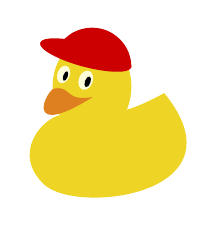
\begin{tikzpicture}
  \duck[cap=red!80!black]
\end{tikzpicture}
%
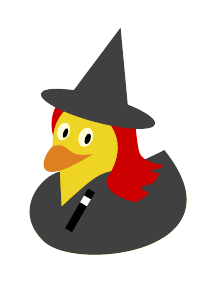
\begin{tikzpicture}
  \duck[witch=black!50!gray,
        longhair=red!80!black,
        jacket=black!50!gray,
        magicwand]
\end{tikzpicture}
%
\definecolor{mggreen}{RGB}{37,166,89}%
\begin{tikzpicture} 
\duck[mohican,tshirt=mggreen,stripes={\stripes},football]
\end{tikzpicture}
%
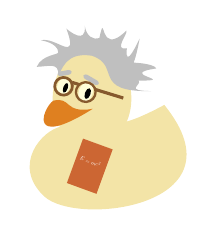
\begin{tikzpicture}
  \duck[body=yellow!50!brown!40!white,
    crazyhair=gray!50!white,
    eyebrow,
    glasses=brown!70!black,
    book=\scalebox{0.2}{$E=mc^2$},
    bookcolour=red!20!brown]
\end{tikzpicture}
%

\begin{tikzpicture}
  \colorlet{skin}{white!45!gray!80!green}
  \duck[lightsaber, body=skin, bill=gray!80!green,
        tshirt=brown!50!black, jacket=brown!30!gray]
  \fill[skin,rounded corners=3] (0.44,1.70) -- (0.25,2) -- (0.6,1.95);
  \fill[skin,rounded corners=3] (1.34,1.60) -- (1.53,1.9) -- (1.16,1.85);
\end{tikzpicture}  
%
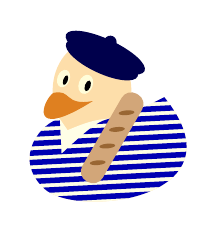
\begin{tikzpicture} 
\duck[body=yellow!60!red!30!white,tshirt=white!90!yellow,stripes={\stripes[color=blue!70!black,rotate=-87,width=0.07,distance=0.12]},beret=blue!30!black,baguette=brown]
\end{tikzpicture}


%
\definecolor{unigold}{RGB}{203,157,52}%
\definecolor{uniblue}{RGB}{46,114,167}%
\definecolor{unired}{RGB}{177,49,34}%
%
\definecolor{skink}{RGB}{245,206,193}%
\definecolor{skins}{RGB}{255,222,151}%
\definecolor{skinu}{RGB}{146,113,96}%
%
\newcommand*{\insignia}{\node[rotate=15] at (wing) {\color{yellow!80!brown}\faLocationArrow};}
%
\begin{tikzpicture}
\duck[tshirt=black!60!gray, jacket=uniblue, body=skins, mullet=black!60!brown, bill=skins!60!gray]
\fill[skins,rotate=175, xshift=-46, yshift=-74] (0.45,1.20)--(0.50,0.80)--(0.65,1.20);
\fill[black!60!brown, rounded corners=1, rotate=70] (1.85,0.13) rectangle (1.91,-0.05);
\fill[black!60!brown, rounded corners=1, rotate=90] (1.7,-0.75) rectangle (1.76,-0.97);
\insignia
\end{tikzpicture}
%
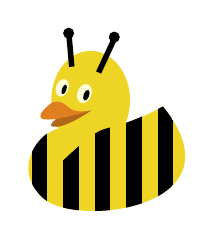
\begin{tikzpicture}
  \duck[stripes={\stripes[distance=0.4,width=0.2,rotate=0,initialx=0.15]},alien=black,laughing]
\end{tikzpicture}  
%
\newcommand{\superstripes}{\stripes[color=blue!80!black,width=3,height=1.0,rotate=5] \stripes[color=blue!80!black,width=0.1,rotate=0,distance=0.7,initialx=-1.1,height=2]}
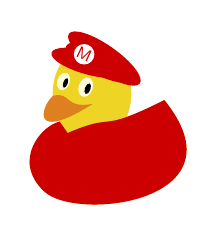
\begin{tikzpicture}
\duck[tshirt=red!80!black,peakedcap=red!80!black,stripes={\superstripes}]
\fill[white] (0.8,2) circle (0.13);
\node[red!80!black,rotate=-25] at (0.8,2) {\scalebox{0.6}{\textsf{M}}};
\end{tikzpicture}  
%
\definecolor{fskin}{RGB}{161,140,126}%
\definecolor{fbill}{RGB}{238,212,191}%
\definecolor{fhair}{RGB}{89,72,72}%
\begin{tikzpicture}
\duck[body=fskin,bill=fbill,shorthair=fhair,bunny,inear=fbill]
\node[fskin,rotate=45,scale=3] at (1.7,1.55) {\textsf{s}};
\fill[fhair,rotate=45] (2.4,0.13) ellipse (0.15 and 0.07); 
\end{tikzpicture}   
%
\hspace*{-1.5em}
%
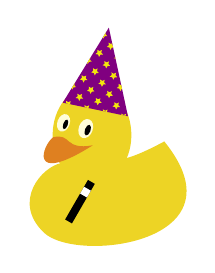
\begin{tikzpicture}
  \duck[magichat,magicwand]
\end{tikzpicture}
%
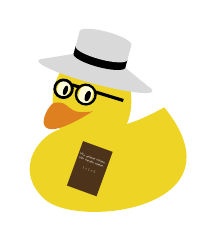
\begin{tikzpicture}
  \duck[glasses,
  bookcolour=black!60!brown,
  book={
      \scalebox{0.14}{
      \parbox{2.5cm}{
      \sffamily
      \centering
      \footnotesize
      Wir m\"ussen wissen.\\
      Wir werden wissen.\\[0.4cm]
      $1+1=2$}}}
  ]
  \fill[gray!30!white,rotate=-15] (0.44,2.0) ellipse (0.75 and 0.1);  
  \fill[gray!30!white,rotate=-15] (0.1,2.05) rectangle (0.78,2.5);
  \fill[gray!30!white,rotate=-15] (0.44,2.5) ellipse (0.34 and 0.08);  
  \fill[gray!30!white,rotate=-15] (-0.3,2.02) -- (1.18,2.02) -- (0.78,2.2) -- (0.1,2.2) -- cycle;
  \fill[black,rotate=-15] (0.44,2.2) ellipse (0.34 and 0.08);   
  \fill[black,rotate=-15] (0.1,2.2) rectangle (0.78,2.3);
  \fill[gray!30!white,rotate=-15] (0.44,2.3) ellipse (0.34 and 0.08);  
\end{tikzpicture}

\end{document}